\everymath{\displaystyle}
\documentclass{beamer}
% \documentclass[handout]{beamer}

%\usepackage[pdftex]{color,graphicx}
\usepackage{amsmath,amssymb,amsfonts}

\mode<presentation>
{
  % \usetheme{Darmstadt}
  % \usetheme[hideothersubsections]{Hannover}
  % \usetheme[hideothersubsections]{Goettingen}
  \usetheme[hideothersubsections, right]{Berkeley}

  \usecolortheme{seahorse}
  % \usecolortheme{dolphin}
  \usecolortheme{rose}
  % \usecolortheme{orchid}

  \useinnertheme[shadow]{rounded}

  \setbeamercovered{transparent}
  % or whatever (possibly just delete it)
}

\mode<handout>{
  \setbeamercolor{background canvas}{bg=black!5}
  \usepackage{pgfpages}
  \pgfpagesuselayout{4 on 1}[a4paper,border shrink=5mm, landscape]
}

\usepackage[brazilian]{babel}
% or whatever

% \usepackage[latin1]{inputenc}
\usepackage[utf8]{inputenc}
% or whatever

\usepackage{times}
%\usepackage[T1]{fontenc}
% Or whatever. Note that the encoding and the font should match. If T1
% does not look nice, try deleting the line with the fontenc.


\title%[] % (optional, use only with long paper titles)
{Análise Exploratória de Dados}

\subtitle
{Formulação de perguntas de dados preliminares} % (optional)

\author%[] % (optional, use only with lots of authors)
{Felipe Figueiredo}% \and S.~Another\inst{2}}
% - Use the \inst{?} command only if the authors have different
%   affiliation.

\institute[INTO] % (optional, but mostly needed)
{Instituto Nacional de Traumatologia e Ortopedia
}
  % \inst{1}%
  % Department of Computer Science\\
  % University of Somewhere
  % \and
  % \inst{2}%
  % Department of Theoretical Philosophy\\
  % University of Elsewhere}
% - Use the \inst command only if there are several affiliations.
% - Keep it simple, no one is interested in your street address.

\date%[] % (optional)
{}

% \subject{Talks}
% This is only inserted into the PDF information catalog. Can be left
% out. 



% If you have a file called "university-logo-filename.xxx", where xxx
% is a graphic format that can be processed by latex or pdflatex,
% resp., then you can add a logo as follows:

\pgfdeclareimage[height=1.6cm]{university-logo}{../logo}
\logo{\pgfuseimage{university-logo}}



% Delete this, if you do not want the table of contents to pop up at
% the beginning of each subsection:
\AtBeginSubsection[]
%\AtBeginSection[]
{
  \begin{frame}<beamer>{Sumário}
    \tableofcontents[currentsection,currentsubsection]
  \end{frame}
}


% If you wish to uncover everything in a step-wise fashion, uncomment
% the following command: 

% \beamerdefaultoverlayspecification{<+->}


\begin{document}

\begin{frame}
  \titlepage
\end{frame}

\begin{frame}{Sumário}
  \tableofcontents
  % You might wish to add the option [pausesections]
\end{frame}


%% Template
% \section{}

% \subsection{}

% \begin{frame}{}
%   \begin{itemize}
%   \item 
%   \end{itemize}
% \end{frame}

% \begin{frame}
%   \begin{columns}
%     \begin{column}{5cm}
%     \end{column}
%     \begin{column}{5cm}
%     \end{column}
%   \end{columns}
% \end{frame}

% \begin{frame}{}
%   \includegraphics[height=0.4\textheight]{file1}
%   \includegraphics[height=0.4\textheight]{file2}
%   \includegraphics[height=0.4\textheight]{file3}
%   \begin{figure}
%     \caption{}
%   \end{figure}
% \end{frame}

% \begin{frame}{}
%   \begin{definition}
%   \end{definition}
%   \begin{example}
%   \end{example}
%   \begin{block}{Exercício}
%   \end{block}
% \end{frame}

\section{Análise Exploratória}

\subsection{EDA}

\begin{frame}{Paradigmas de Análises de Dados}
Estudos quantitativos exigem coleta e análise de dados
  \begin{itemize}
  \item EDA -- Análise Exploratória de Dados
  \item CDA -- Análise Confirmatória de Dados
  \end{itemize}
\end{frame}

\begin{frame}{Análise Exploratória de Dados}
  \begin{itemize}
  \item<1-> Formalizado por John W. Tukey nos anos 1970
  \item<1-> Objetivo: formular perguntas com base nos dados disponíveis
  \item<2-> Perguntas que podem ser respondidas pela análise dos dados
  \end{itemize}
\end{frame}

\begin{frame}{Análise Exploratória de Dados}
  \begin{block}{O que é}
    EDA é uma filosofia/approach para
    \begin{itemize}
    \item maximizar a compreensão/insight sobre um dataset
    \item descobrir estruturas
    \item identificar variáveis importantes
    \item detectar outliers e anomalias
    \end{itemize}
  \end{block}
  Fonte: NIST Handbook (1998)
\end{frame}

\begin{frame}{Análise Exploratória de Dados}
  \begin{block}{Tukey, 1980}
    {\em ``Ideas come from previous exploration more often than from
      lightning strokes. Important questions can demand the most
      careful planning for confirmatory analysis. (\ldots) Finding the
      question is often more important than finding the
      answer. Exploratory data analysis is an atitude, (\ldots) NOT a
      bundle of techniques (\ldots).''}
  \end{block}

Tukey (1980) - We Need Both Exploratory and Confirmatory
\end{frame}

\begin{frame}{Análise Exploratória de Dados}
  Para Tukey:
  \begin{itemize}
  \item Não basta fazer a análise confirmatória, nem a exploratória:
    \alert{ambas} são necessárias
  \item Paradigma: pergunta $\rightarrow$ resposta é inadequado
  \item ``Encontrar a pergunta é por vezes mais importante que
    encontrar a resposta''
  \end{itemize}
\end{frame}

\begin{frame}{Paradigma linear}
  \begin{center}
    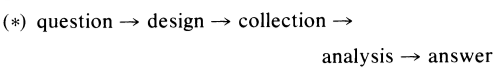
\includegraphics[width=0.7\textwidth]{EDA/eda-tukey1}
  \end{center}
  \begin{enumerate}
  \item Como as perguntas são geradas?
  \item Como os desenhos (experimentais) são guiados?
  \item Como a coleta de dados é monitorada?
  \end{enumerate}
\end{frame}

\begin{frame}{Questões sobre o paradigma confirmatório}
  Respostas: Geralmente por \ldots
  \begin{enumerate}
  \item  {\em insights} teóricos e a exploração de dados
    anteriores (e.g., pesquisa bibliográfica)
  \item informação qualitativa disponível obtida da exploração de
    dados anteriores
  \item exploração dos dados, conforme são obtidos, buscando
    comportamento ``inesperado''
  \end{enumerate}
\end{frame}

\begin{frame}{Explorar\ldots}
  \begin{itemize}
  \item A chave então é explorar os dados
  \item Explorar antes, durante e depois da análise confirmatória
  \item Busca de pistas, idéias e eventualmente conclusões
    preliminares ({\em hipóteses}!)
  \end{itemize}
\end{frame}

\begin{frame}{Paradigma alternativo}
  \begin{center}
    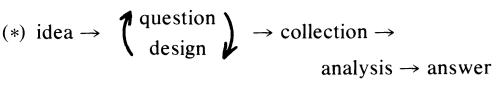
\includegraphics[width=0.7\textwidth]{EDA/eda-tukey2}
  \end{center}

Tukey sugere que:
  \begin{itemize}
  \item Antes de termos uma pergunta, temos uma idéia (a ser
    formalizada)
  \item Pergunta formal depende dos dados disponíveis
  \item Questão pragmática, independe do desejo ou vontade
  \end{itemize}
\end{frame}

\begin{frame}{Exemplo}
  \begin{example}
    \begin{itemize}
    \item Idéia: uma certa droga ajuda em uma doença
    \item<2-> Queremos testar/confirmar isso\ldots
    \item<3-> \ldots com consistência estatística na resposta
    \end{itemize}
  \end{example}
  \begin{itemize}
  \item Idéia preliminar informal, vaga
  \item Geralmente em termos de linguagem coloquial
  \item Não pode ser avaliada com suporte estatístico
  \end{itemize}
\end{frame}

\begin{frame}{Exemplo}
Desejo: pergunta geral, de amplo espectro e implicações profundas
\begin{example}
  ``Dos pacientes que morreriam em até três anos desta doença, que
  fração poderia ser salva por este tratamento?''
\end{example}
\begin{itemize}
\item Dificuldade técnica\ldots
\item \ldots nenhum design pode isolar essas pessoas para um experimento
\end{itemize}
\end{frame}

\begin{frame}{Exemplo}
  O que \alert{pode} ser perguntado está limitado por:
  \begin{itemize}
  \item Idade e sexo dos pacientes
  \item conjunto mínimo de sintomas
  \item ausência de outras condições potencialmente fatais
  \item tipos de pacientes que podem ser encontrados/observados
  \item etc.
  \end{itemize}
\end{frame}

\begin{frame}{Formulação da pergunta}
  \begin{itemize}
  \item o que pode concretamente ser perguntado
  \item que desenhos são viáveis
  \item chance de um certo design resultar em resposta útil
  \item ``Como eu estudo o que está acontecendo aqui?''
  \end{itemize}
\end{frame}

\begin{frame}{Por onde começar?}
  \begin{itemize}
  \item tabelas
  \item gráficos dos dados brutos
  \item estatísticas descritivas simples
  \item procurar padrões
  \end{itemize}
\end{frame}

\subsection{Gráfico de Dispersão}

\begin{frame}{Gráficos de dispersão}
Gráficos de dispersão (ou scatter-plots):
  \begin{itemize}
  \item visualizar os dados pontuais diretamente
  \item identificar possíveis padrões ou tendências
  \item identificar visualmente possíveis outliers
  \item desenhar possíveis relações (modelos) sobre os dados
  \end{itemize}
\end{frame}

\begin{frame}
  \begin{center}
    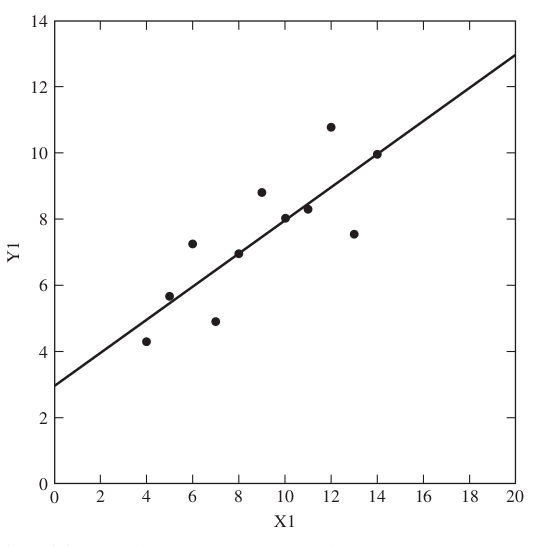
\includegraphics[height=0.7\textheight]{EDA/eda-dispersao1}
  \end{center}
  Fonte: Behrens, Yu (2003)
\end{frame}

\begin{frame}
  \begin{center}
    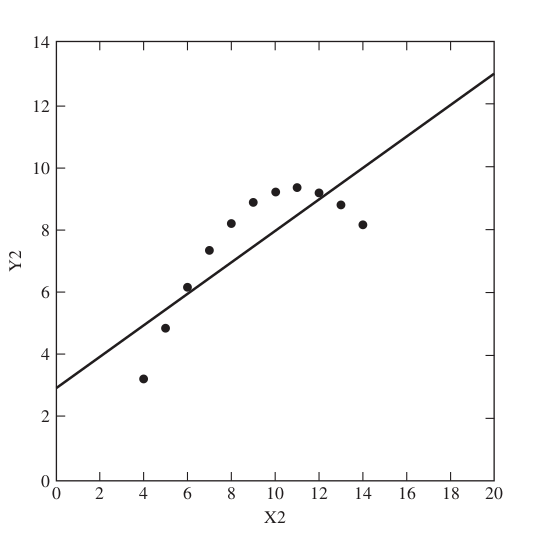
\includegraphics[height=0.7\textheight]{EDA/eda-dispersao2}
  \end{center}
  Fonte: Behrens, Yu (2003)
\end{frame}

\begin{frame}
  \begin{center}
    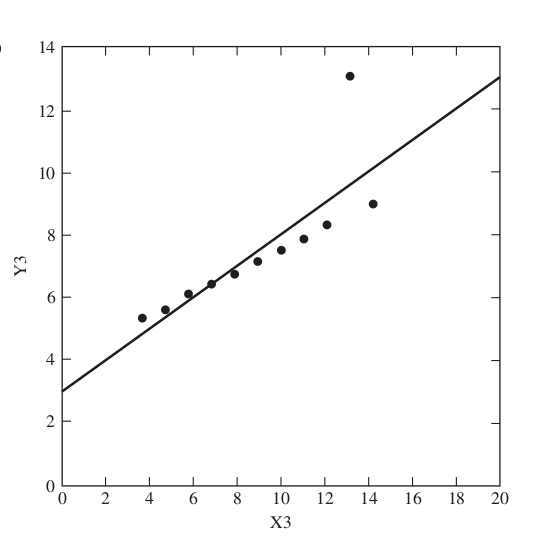
\includegraphics[height=0.7\textheight]{EDA/eda-dispersao3}
  \end{center}
  Fonte: Behrens, Yu (2003)
\end{frame}

\begin{frame}
  \begin{center}
    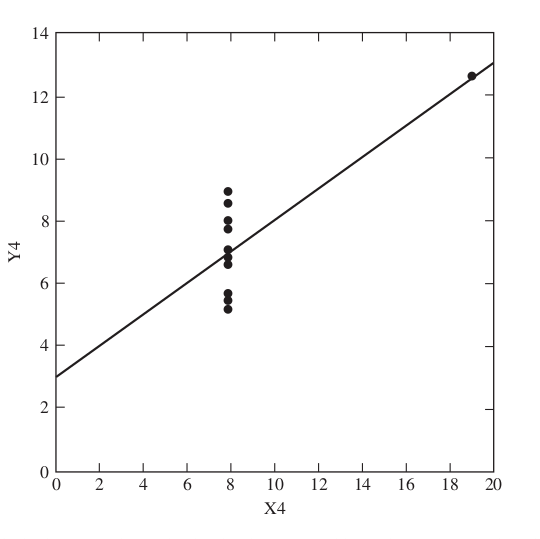
\includegraphics[height=0.7\textheight]{EDA/eda-dispersao4}
  \end{center}
  Fonte: Behrens, Yu (2003)
\end{frame}

\subsection{Histogramas}

\begin{frame}{Histograma}
  \begin{itemize}
  \item Gráfico de barras com frequências dos dados
  \item visualização prática da distribuição dos dados
  \item identificar simetria, tendência central, dispersão, etc
  \end{itemize}
\end{frame}

\begin{frame}
  \begin{center}
    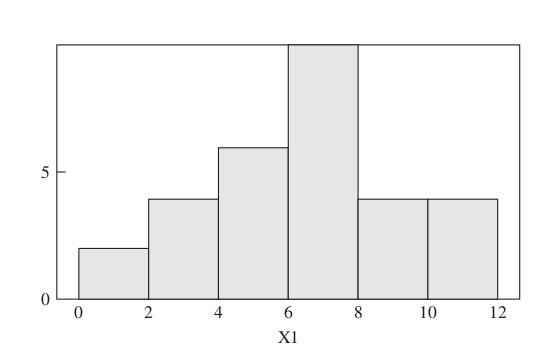
\includegraphics[height=0.7\textheight]{EDA/eda-histograma1}
  \end{center}
  Fonte: Behrens, Yu (2003)
\end{frame}

% \begin{frame}
%   \begin{center}
%     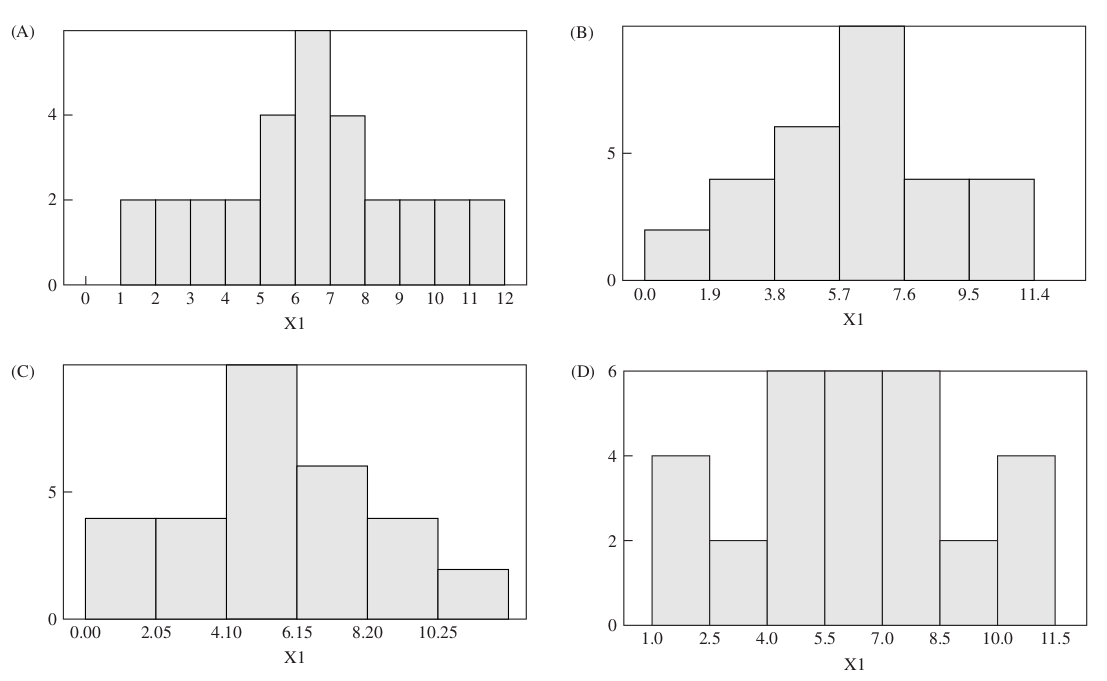
\includegraphics[width=1\textwidth]{EDA/eda-histograma2}
%   \end{center}
%   Fonte: Behrens, Yu (2003)
% \end{frame}

\subsection{Boxplot}

\begin{frame}{Boxplot}
  \begin{itemize}
  \item caixa que contém 50\% dos dados\ldots
  \item \ldots e segmentos verticais que englobam a maior parte dos
    dados
  \item elementos fora deste intervalo devem ser investigados como
    possíveis outliers
  \end{itemize}
\end{frame}

\begin{frame}
  \begin{center}
    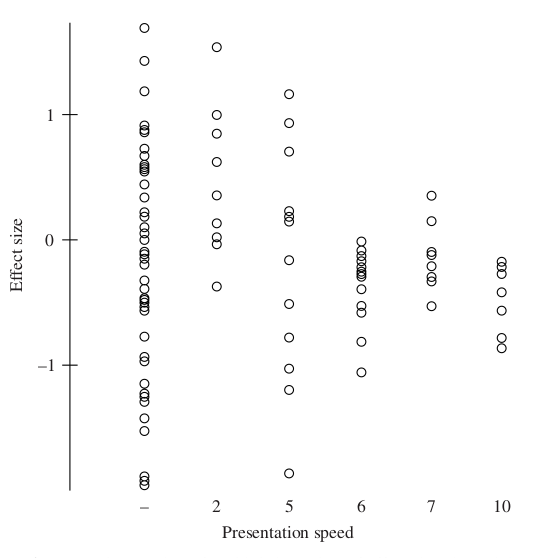
\includegraphics[height=0.7\textheight]{EDA/eda-boxplot1}
  \end{center}
  Fonte: Behrens, Yu (2003)
\end{frame}

\begin{frame}
  \begin{center}
    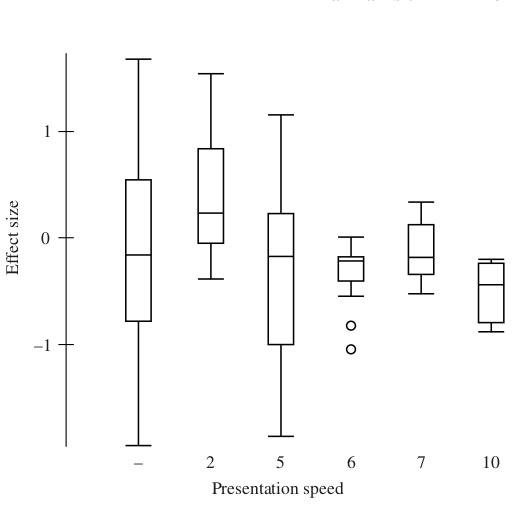
\includegraphics[height=0.7\textheight]{EDA/eda-boxplot2}
  \end{center}
  Fonte: Behrens, Yu (2003)
\end{frame}

\subsection{Referências}

\begin{frame}{Referências}
  \begin{itemize}
  \item<1-> NIST Handbook (1998), Exploratory Data Analysis, cap 1 -
    \url{http://www.itl.nist.gov/div898/handbook/eda/section1/eda1.htm}
    (Acessado em 10/09/2015)
  \item<1-> Tukey (1980), We need both exploratory and confirmatory,
    \url{http://www-ece.rice.edu/~fk1/classes/ELEC697/TukeyEDA.pdf}
    (Acessado em 10/09/2015)
  \item<1-> Behrens, Yu (2003), Exploratory Data Analysis, cap 2 -
    Research Methods in Psychology
  \end{itemize}
\end{frame}
\end{document}
